\documentclass[../main-manifolds.tex]{subfiles}

\begin{document}
\providecommand{\szz}{\mathcal{S}}
\providecommand{\ccinf}{C_c^\infty}

% Topologies
\providecommand{\Taux}{\Tau_\xx}
\providecommand{\Tauy}{\Tau_\yy}
\providecommand{\Tauxy}{\Tau_{\xx\times\yy}}

% Basis
\providecommand{\Bx}{\borel_\xx}
\providecommand{\By}{\borel_\yy}
\providecommand{\Bxy}{\borel_{\xx\times\yy}}


\fchapter{1: Topological Manifolds}
\newpage
\topheader{Topological Manifolds}
The study of differential geometry begins with tens of pages of definitions.
\begin{definition}[Topological Manifold]\label{lee-chp1:topological-manifold-definition}
    Let $M$ be a topological space. $M$ is a topological manifold of dimension $m$ if it is Hausdorff, second-countable, and locally homeomorphic to $\realn$.
\end{definition}

\begin{definition}[Local homeomorphism]\label{lee-chp1:locally-homeomorphic-definition}
    $M$ locally homeomorphic to $\realn$ if every point $x\in M$ an open set $U$, equipped with a homeomorphism which sends points in $U$ into an open subset of $\realn$. 
    \[
        \phi: U\to \phi(U)
    \] 
    The tuple $(U,\phi)$ is called a coordinate chart.
\end{definition}

\begin{definition}[More on coordinate charts]\label{lee-chp1:coordinate-chart-definition}
    \begin{itemize}
        \item A coordinate chart $(U,\phi)$ is centered at $p\in M$ if $p\in U$ and $\phi(p)=0\in\realn$.
        \item We call $U$ the coordinate domain, and
        \item we call $\phi$ the coordinate map.
        \item If the choice of $(U,\phi)$ is unambiguous, then the local coordinates of $p$ are simply the coordinates of $\phi(p)$ in $\realn$, and
        \item we sometimes also denote $\phi(U)$ by $\hat{U}$ if it is unambiguous to do so.
        \item If $\hat{U}$ is an open ball/cube, then $U$ is called a coordinate ball/cube.
    \end{itemize}
\end{definition}

The central theme of point-set topology (or even metric topology) is that of passing a topological argument to the basis or to a neighbourhood. Manifolds in particular have a nice basis.
\begin{wts}[Basis of precompact coordinate balls]
    Every topological manifold has a countable basis of precompact coordinate balls.
\end{wts}
\begin{wts}[Additional facts about topological manifolds]
If $M$ is a topological manifold, 
\begin{itemize}
    \item $M$ is locally compact. (Lee, Proposition 1.12)
    \item $M$ is paracompact, and every open cover has a refinement 
    that is another countably locally finite open cover whose elements are chosen from an arbitrary (but fixed) basis of $M$. (Lee, Theorem 1.15)
    \item $M$ is locally-path connected.
    \item $M$ is connected iff it is path-connected.
    \item $M$ is metrizable. (Munkres Chapter 6)
\end{itemize}
\end{wts}

\topheader{Smooth Manifolds}
We wish to perform calculus on manifolds.
\begin{definition}[Smooth function $F:\realn\to\realm$]\label{lee-chp1:real-smooth-function}
    Let $F:\realn\to\realm$, replacing $\realn$ and $\realm$ with open subsets if necessary. $F$ is smooth if its (scalar-valued) component functions has continuous partial derivatives of all orders. The set of smooth functions from $\realn$ to $\realm$ is sometimes denoted by $\cinf[\realn,\realm]$. If $m=1$, we sometimes write $\cinf[\realn]$, similar to a test function on the Schwartz Space.
\end{definition}

\begin{definition}[Transition map from $\phi$ to $\psi$]\label{lee-chp1:transition-maps}
    Let $(U,\phi)$ and $(V,\psi)$ be coordinate charts on $M$. The composite function (whenever $U\cap V\neq\varnothing$) 
    \[
    \psi\circ\phi^{-1}:\phi(U\cap V)\to\psi(U\cap V)
    \] 
    is called the transition map. Notice $\psi\circ\phi^{-1}$ is by definition a homeomorphism.
\end{definition}

\begin{definition}[Smoothly compatiable]\label{lee-chp1:smoothly-compatible}
    Two coordinate charts on $M$, $(U,\phi)$ and $(V,\psi)$ are called smoothly compatible if either their domains are disjoint, or their transition map is a diffeomorphism on $\realm$.
\end{definition}

\begin{definition}[Smooth atlas]\label{lee-chp1:smooth-atlas}
    An atlas $\acal$ of $M$ is a collection of charts $\{(U_\alpha, \phi_\alpha)\}$ whose collection of coordinate domains $\{U_\alpha\}$ for an open cover of $M$.\\ It is called a smooth atlas if any two charts in the atlas are pairwise smoothly compatible.
\end{definition}

\begin{definition}[Smooth manifold]\label{lee-chp1:smooth-manifold}
    A smooth atlas $\acal$ on $M$ is maximal if it is not contained (properly) in any other smooth atlas as a subset. In other words, if $(U',\phi')$ is a chart on $M$ that is smoothly compatible with all elements in $\acal$, then $(U',\phi')\in\acal$ already.\\
    
    This smooth atlas is often very large, it includes all translations of charts, dilations, and composition with diffeomorphisms in $\realm$, restrictions onto open subsets, etc. A maximal smooth atlas is sometimes called a complete atlas, or a smooth manifold structure.\\

    A smooth manifold is the tuple $(M,\acal)$, where $\acal$ is some smooth atlas. It can happen if $M$ is originally a topological manifold with a huge number of charts, some of which are smoothly compatible with others, that $\acal$ is a strict subset, and both $\acal_1$ and $\acal_2$ are maximal smooth atlases on $M$, but $\acal_1\neq\acal_2$. We often omit $\acal$ and write $M$ if the smooth atlas is understood or not of importance.
\end{definition}

\begin{definition}[Smooth coordinate terminologies]\label{lee-chp1:smooth-coordinate-definitions}
    Let $(M,\acal)$ be a smooth manifold. 
    \begin{itemize}
        \item Any coordinate chart $(U,\phi)\in\acal$ is called a smooth chart, similar to \cref{lee-chp1:coordinate-chart-definition}
        \item We call $U$ the \emph{smooth coordinate domain} or \emph{smooth coordinate neighbourhood} of any $p\in U$, and
        \item we call $\phi$ the \emph{smooth coordinate map}.
        \item The terms \emph{smooth coordinate ball} and \emph{smooth coordinate cube} are used similarly.
        \item A set $B\subseteq M$ is a \emph{regular coordinate ball} if its image is a smooth coordinate ball centered at the origin; and the closure of this ball in $\realm$ is a subset of the image of another smooth coordinate ball, centered at the origin.
    \end{itemize}
\end{definition}

\begin{definition}[Standard smooth structure on $\realn$]\label{lee-chp1:standard-smooth-structure-realn}
    The maximal smooth atlas containing $(\realn,\id{\realn})$ is called the \emph{standard smooth structure on $\realn$}.
\end{definition}

Manifolds with boundary are not as important as regular manifolds for now, but they are worth mentioning.
\begin{definition}[Closed n-dimensional upper half-plane $\halfn\subseteq\realn$]\label{lee-chp1:upper-half-plane-definitions}
    We define the following symbols for the upper half plane.
    \begin{itemize}
        \item $\halfn = \bigset{x\in\realn,\: x^n\geq 0}$,
        \item $\Int\halfn = \bigset{x\in\realn,\: x^n > 0}$,
        \item $\partial\halfn = \bigset{x\in\realn,\: x^n = 0}$
    \end{itemize}
\end{definition}
\begin{definition}[Manifolds with boundary]\label{lee-chp1:manifolds-with-boundary-definition}
    A topological space $M$ is called a manifold with boundary if it is Hausdorff, second-countable, and locally homeomorphic to an open subset of $\halfn$ (endowed with the subspace topology from $\realn$).\\

    A chart $(U,\phi)$ is an \emph{interior chart} if its coordinate image is disjoint from the 'boundary' of the upper-half plane. This means $\phi(U)\cap \partial\halfn=\varnothing$. Similarly, $(V,\psi)$ is a \emph{boundary chart} if its range contains a point in $\partial\halfn$; so $\psi(V)\cap\partial\halfn\neq\varnothing$.\\

    Similar to \cref{lee-chp1:coordinate-chart-definition} and \cref{lee-chp1:smooth-coordinate-definitions}, we use the terms \emph{coordinate half-ball}, \emph{coordinate half-cube}, \emph{regular coordinate half-ball}.\\

    Let $p\in M$, it is called an \emph{interior point of $M$} (not to be confused with the topological interior) if it is in the domain of some interior chart, and $p$ is called a \emph{boundary point of $M$} if there exists a boundary chart that sends $p$ into $\partial\halfn$. The set of interior points and boundary points of $M$ will be denoted by $\Int M$ and $\partial M$.
\end{definition}

\newpage

\begin{example}[Sphere as a topological manifold]
    The $n$-sphere as a topological manifold. Define 
\[
    S^n = \bigset{x\in\real^{n+1},\: |x|=1}
\]
We claim that $\{U_i^{\pm}\}_{i=1}^{n+1}$ form an open cover, where
\[
    U_i^+ = \bigset{x\in S^n, x^i>0}\quad U_i^- = \bigset{x\in S^n, x^i<0}
\]
Each $U_i^{\pm}$ is the inverse image of $\pnv{i}{(0,+\infty)}\cap S^n$ or $\pnv{i}{(0,-\infty)}\cap S^n$, hence open. For every $x\in S^n$, there exists at least some $1\leq j\leq n+1$ that makes the $j$-th coordinate of $x$, $x^j\neq 0$. So 
\[
    S^n = \bigcup_{i}U_i^\pm
\]
Denote the unit ball $\bigset{x\in\realn,\: |x|<1}$ in $\realn$ by $\borel^n$. 

\end{example}

\newpage

\fchapter{2: Smooth Maps}\newpage

\topheader{Smooth Maps}

\begin{definition}[Smooth functions {$\cinf[M,\real^k]$}]\label{lee-chp2:test-functions-on-manifolds}
    Let $F: M\to\real^k$ be a vector-valued function on a smooth manifold $M$. We say $F$ is a smooth function if for every $p\in M$, there exists a smooth chart $p\in (U,\phi)$ such that the \emph{coordinate representation of $F$ at $p$, with respect to $(U,\phi)$} is a smooth function from $\realm$ to $\real^k$, denoted by $\hat{F}$ (in the sense of \Cref{lee-chp1:real-smooth-function}).
    \[
        \hat{F}=F\circ \phi^{-1}:\phi(U)\to\real^k\in \cinf[\phi(U),\realk]
    \]
    if $k=1$, then we denote the space of \emph{test functions} on $M$ by $\cinf[M]=\cinf[M,\real]$
\end{definition}

\begin{definition}[Smooth maps between manifolds {$\cinf[N,M]$}]\label{lee-chp2:smooth-maps-between-manifolds-definition}
    Let $F:N\to M$ be a map between smooth manifolds $N$ and $M$ (note we switched the order). $F$ is a smooth map if at every $p\in M$, there exists 
    \begin{itemize}
        \item a chart in the smooth atlas of $N$ (the domain), $p\in (U,\phi)$,
        \item another chart in the smooth atlas of $M$ (the range), $F(U)\subseteq(V,\psi)$,
        \item such that, the \emph{coordinate representation of $F$ at $p$ with respect to $(U,\phi)$, and $(V,\psi)$} is a smooth function from $\realn$ to $\realm$, also denoted by $\hat{F}$.
        \begin{equation}\label{lee-chp2:eq-smooth-map-coordinate-representation}
            \hat{F} = \psi\circ F\circ \phi^{-1}:\phi(U)\to \psi(V)\in \cinf[\realn,\realm]
        \end{equation}
    \end{itemize}
\end{definition}

The following propositions summarizes common operations on smooth maps, a few sources of them.
\begin{wts}[Smooth maps are continuous]\label{lee-chp2:smooth-maps-are-continuous}
    If $F:N\to M$ is a smooth map, then $F$ is continuous with respect to the topologies on $N$ and $M$.
\end{wts}
\begin{proof}
    Let $p\in N$ be fixed, because $F$ is smooth this induces two smooth charts, one in the domain and another in the range; as in \cref{lee-chp2:smooth-maps-between-manifolds-definition}. $F(p)$ is a point in $M$. From \cref{lee-chp2:eq-smooth-map-coordinate-representation}, $\hat{F}|\phi(U)$ is a smooth hence continuous function. Since $\phi: U\mapsto \phi(U)$ and $\psi: V\mapsto \psi(V)$ are homeomorphisms, 
    \[
        F|U = \underbracket{\psi^{-1}}_{\text{continuous}}\circ \underbracket{\hat{F}|\phi(U)}_{\text{smooth}}\circ \underbracket{\phi}_{\text{continuous}}\qq{is continuous on }U
    \]
    Let the point $p$ range through all the points in $N$, so $F$ is continuous at every $p$, hence on $N$.
\end{proof}
\begin{wts}[Characterizations of Smooth Maps in {$\cinf[N,M]$}]\label{lee-chp2:characterizations-of-smooth-maps}
    Let $N$ and $M$ be smooth manifolds, and $F:N\to M$. $F$ is a smooth map iff
    \begin{itemize}
        \item For every $p\in N$, there exists smooth charts $p\in (U,\phi)$ and $F(p)\in (V,\psi)$ such that $U\cap F^{-1}(V)$ is an open set in $N$, and the composite map (the coordinate representation)
        \[
            \psi\circ F\circ \phi^{-1}|(U\cap F^{-1}(V)):\phi(U\cap F^{-1}(V))\to \psi(V)\qq{is smooth}
        \]
        \item $F$ is continuous and there exist smooth atlases $\{(U_\alpha,\phi_\alpha)\}\subseteq\acal_N$, and $\{(V_\beta,\psi_\beta)\}\subseteq\acal_M$ such that the coordinate representation 
        \[
            \psi_\beta\circ F\circ \phi_\alpha^{-1}:\phi(U_\alpha\cap F^{-1}(V_\beta))\to \psi(V_\beta)\qq{is smooth}
        \]
        whenever it makes sense.
        \item the restriction of $F$ onto any arbitrary open set $U$, $F|U: U\mapsto M$ is smooth (in the sense of open submanifold).
    \end{itemize}
\end{wts}
\begin{proof}
    By \Cref{lee-chp2:smooth-maps-are-continuous}, and the fact that complete atlases are closed under restrictions onto open sets, it is clear that the original definition implies the two. The first definition also clearly implies the original definition, as we can restrict 
    
    \[(U,\phi)\mapsto \biggl(U\cap F^{-1}(V),\: \phi\eval_{U\cap F^{-1}(V)}\biggr)\]
    
    since $U\cap F^{-1}(V)$ is open in the domain manifold.\\

    The second definition implies the original one as well, since the smooth atlases are taken from the maximal atlas, we can pass the argument to any smoothly-compatible chart. Atlases must cover both the domain and the range, and coordinate transitions between smoothly compatible charts are diffeomorphisms. If $F$ is smooth on a subcollection of those charts, meaning
    \[
        \psi_\beta\circ F\circ\phi_\alpha^{-1}\in \cinf[\phi_\alpha(U_\alpha)\cap F^{-1}(V_\beta),\psi_\beta(V_\beta)]
    \]
    it is smooth with respect to every pair of (smooth) charts in the two atlases $\acal_{N}$, $\acal_{M}$, as a composition of smooth maps:
    \[
        \psi\circ \underbracket{\psi^{-1}\circ \psi_\beta}_{\text{smooth}}\circ F\circ\underbracket{\phi_\alpha^{-1}\circ \phi}_{\text{smooth}}\circ\phi^{-1}
    \]
    where we can restrict $\phi_\alpha\mapsto \phi_\alpha|(U_\alpha\cap F^{-1}(V_\beta))$ by continuity of $F$.

    I will prove the third and last equivalence later.
\end{proof}
\begin{wts}[Sources of smooth maps]\label{lee-chp2:sources-of-smooth-maps}
    Let $N$, $M$, $P$ be smooth manifolds, then
    \begin{itemize}
        \item Every constant map is smooth,
        \item The identity map $\id{M}:M\to M$ is smooth,
        \item The inclusion map $\iota: W\to M$ is smooth, where $W$ is an open submanifold of $M$.
        \item The composition of smooth maps is again a smooth map: if $F\in \cinf[N,M]$ and $G\in \cinf[M,P]$, then $(G\circ F)\in\cinf[N,P]$
    \end{itemize}
\end{wts}

\topheader{Diffeomorphisms}
\begin{definition}[Diffeomorphism between Manifolds $\mathcal{D}(N,M)$]\label{lee-chp2:diffeomorphism-definition}
    Let $N$ and $M$ be smooth manifolds, $F:N\to M$ is a diffeomorphism if it is a smooth bijective map with a smooth inverse. We denote the space of diffeomorphisms from $N$ to $M$ by $\diffeo[N,M]$.
\end{definition}

\begin{wts}[Properties of Manifold Diffeomorphisms]\label{lee-chp2-diffeomorphism-properties}
    Let $N$, $M$ and $P$ be smooth manifolds, then
    \begin{itemize}
        \item The composition of diffeomorphisms is again a diffeomorphism, that is, if $F\in \diffeo[N,M]$ and $G\in \diffeo[M,P]$, then $(G\circ F)\in \diffeo[N,P]$.
        \item The open-manifold restriction of a diffeomorphism onto its image is again a diffeomorphism,
        \item Every diffeomorphism is a homeomorphism and an open map.
    \end{itemize}
\end{wts}
\begin{proof}
    Trivial.
\end{proof}

\topheader{Partitions of Unity}
See Folland Chapters 4 and 8. Including Urysohn's Lemma, Tietze's Extension Theorem, the usual construction of $\ccinf$ bump functions.
\newpage

\fchapter{3: Tangent Spaces}\newpage
\topheader{Algebra of Germs on $\cinf[N]$}
The tangent space is a powerful concept that acts almost like the dual in distribution theory.
\begin{definition}[Algebra of Germs at $p$: $C_p^\infty(N)$]\label{lee-chp3:algebra-of-germs-at-p}
    Let $N$ be a smooth manifold and $p\in N$. We define an equivalence relation on the space of test functions on $N$, $\cinf[N]$. If $f,g\in\cinf[N]$, we write $f\sim g$ if $f=g$ for some open neighbourhood about $p$. We denote this equivalence class by $C_p^\infty(N)$, and it is clear $\cinf[N]$ is closed under pointwise multiplication by the product rule, and form an algebra; so $C_p^\infty(N)$ is an algebra too.
\end{definition}

\topheader{Tangent spaces of manifolds}
\begin{definition}[Vector space of derivations at $p$: $T_p N$]\label{lee-chp3:vector-space-of-derivations-at-p}
    Let $\nu: C_p^\infty(N)\to\real$ be a linear functional on the vector space of germs at $p$. It is called a derivation at $p$ if it satisfies the product rule, if $f,g\in C_p^\infty(N)$, 
    \[
        \nu(fg)=g(p)\nu(f)+f(p)\nu(g)
    \]
    then we say 
    \begin{itemize}
        \item $\nu$ is a tangent vector at $p$, 
        \item $\nu\in T_p N$,
        \item $\nu$ is an element of the \emph{tangent space at $p$}.
        \item $\nu$ is a derivation on $N$ at $p$.
    \end{itemize}
\end{definition}
\begin{wts}[Properties of derivations at $p$]
    Let $N$ be a smooth manifold and $p\in N$.
    \begin{itemize}
        \item If $f\in C^\infty_p$ is constant in some neighbourhood of $p$, then $\nu(f)=0$ for every $\nu\in T_pN$,
        \item If $f(p)=g(p)=0$, then $\nu(fg)=0$ for tangent vector $\nu$ at $p$.
    \end{itemize}
\end{wts}

\topheader{Tangent spaces of $\realn$}

\begin{wts}[Basis of $T_p\realn$]
    Let $\realn$ be equipped with the standard smooth structure as in \Cref{lee-chp1:standard-smooth-structure-realn}. The vector space of derivations at $p\in\realn$ are spanned by the $n$ partial derivatives at $p$
    \[
        \eval{\pdv{x^j}}_{p}:f\mapsto \eval{\pdv{x^j}f(x)}_{p},\quad 1\leq j\leq n,\: f\in \cinf[\realn]
    \]
    Moreover, the $n$ vectors form a basis, and $\dim T_p\realn= n$.
\end{wts}
\begin{definition}[Standard Basis of $T_p\realn$]
    The standard basis for the tangent space at $p\in\realn$ is the $n$ partial derivatives at $p$.
    \begin{equation}\label{lee-chp3:standard-basis-for-tangent-space-realn}
        T_p\realn = \bigset{\eval{\pdv{x^1}}_{p},\ldots,\eval{\pdv{x^n}}_{p}}
    \end{equation}
\end{definition}

\begin{definition}[Coordinate functions $x^j$ on $\realn$]
    Let $x^1,\ldots x^n$ be the standard coordinates on $\realn$. If $1\leq j\leq n$, $x^j$ is a function (also represented by the same symbol as the standard coordinate) from $\realn$ to $\real$, which maps each $p = (p^1,\ldots,p^j,\ldots, p^n)$ to its $j$-th coordinate $p\mapsto p^j$.\\

    This map is linear, hence smooth, has the matrix representation of $\mcal\{x^j\}=(\delta_{jk})_{1,k}\in \real^{1\times n}$ where $\delta_{jk}$ denotes the discrete mass at $j$.\\

    Furthermore, the coordinate functions behave like the dual basis for the derivations $\eval{\partial/\partial x^j}_p$ at $p$
    \[
        \eval{\pdv{x^j}}_{p}(x^k) = \delta_{jk}
    \]
    If $\nu\in T_p\realn$, and has the basis representation
    \[
        \nu = \sum_{j}\nu^j\eval{\pdv{x^j}}_{p} = \nu^j\eval{\pdv{x^j}}_{p}
    \]
    then 
    \begin{equation}\label{lee-chp3:derivation-in-realn-projection-using-coordinate-functions}
        \nu = \sum_j \nu(x^j)\eval{\pdv{x^j}}_{p} = \nu(x^j)\eval{\pdv{x^j}}_{p}
    \end{equation}
\end{definition}

\topheader{Differential of a smooth map $F\in \cinf[N,M]$}
\begin{definition}[Differential of a smooth map $dF_p: T_pN\to T_{F(p)}M$]
    Let $F\in\cinf[N,M]$, $p\in N$ and $\nu\in T_pN$ be a tangent vector at $p$. The differential of a smooth map is a linear map that sends tangent vectors in $T_pN$ to tangent vectors in $T_{F(p)}M$. If $f\in \cinf[M]$ is a test function on $M$, then $f\circ F$ is a test function on $N$, and
    \[
        dF_p(\nu)(f) = \nu\biggl(\underbracket{f\circ F}_{\cinf[N]}\biggr)
    \]
\end{definition}
We state the following without proof, as the proof is tedious. It simply involves unboxing the definition of the differential $dF_p: T_pN\to T_p M$, and projecting onto the coordinates.
\begin{wts}[Properties of the differential]\label{lee-chp3:properties-of-differential}
    Let $N$, $M$ and $P$ be smooth manifolds, if $F\in\cinf[N,M]$, $G\in \cinf[M,P]$ then
    \begin{itemize}
        \item $dF_p$ is a linear map between $T_p$ and $T_{F(p)}N$,
        \item $d(G\circ F)_p = dG_{F(p)}\circ dF_p$
        \item $d({\id{N}})_p=\id{T_pN}$,
        \item if $F\in\diffeo[N,M]$, then $dF_p$ is a linear isomorphism between $T_pN$ and $T_{F(p)}M$, and
        \[
            (dF_p)^{-1}=d(F^{-1})_{F(p)}
        \]
    \end{itemize}
\end{wts}

\begin{wts}[Matrix representation of the differential of $F: N\to M$]
Let $F\in \cinf[N,M]$, and $p\in N$ induces two charts $p\in (U,\phi)$ and $F(p)\in(V\,\psi)$. The matrix representation of the differential at $p$, $dF_p: T_p N\to T_{F(p)}M$ is nothing but the Jacobian matrix of size $m\times n$ of the coordinate representation at $p$.
\begin{equation}\label{lee-chap3:jacobian-matrix-representation}
        \mcal\{dF_p\} = \begin{bmatrix}\eval{\pdv{\hat{F}^1}{x^1}}_{\phi(p)} & \eval{\pdv{\hat{F}^1}{x^2}}_{\phi(p)} & \cdots & \cdots & \eval{\pdv{\hat{F}^1}{x^n}}_{\phi(p)} \\[1em] \eval{\pdv{\hat{F}^2}{x^1}}_{\phi(p)} & \eval{\pdv{\hat{F}^2}{x^2}}_{\phi(p)} & \cdots & \cdots & \eval{\pdv{\hat{F}^2}{x^n}}_{\phi(p)} \\[1em] \vdots & \vdots & \vdots & \vdots & \vdots \\[1em] \vdots & \vdots & \vdots & \vdots & \vdots \\[1em] \eval{\pdv{\hat{F}^m}{x^1}}_{\phi(p)} & \eval{\pdv{\hat{F}^m}{x^2}}_{\phi(p)} & \cdots & \cdots & \eval{\pdv{\hat{F}^m}{x^n}}_{\phi(p)}\end{bmatrix}
\end{equation}

Alternately, if we write $\hat{p} = \phi(p)$ as the $\realm$ coordinates at $p$, then

\begin{equation}\label{lee-chap3:jacobian-matrix-representation-alternate}
        \mcal\{dF_p\} = \begin{bmatrix}\eval{\pdv{\hat{F}^1}{x^1}}_{\hat{p}} & \eval{\pdv{\hat{F}^1}{x^2}}_{\hat{p}} & \cdots & \cdots & \eval{\pdv{\hat{F}^1}{x^n}}_{\hat{p}} \\[1em] \eval{\pdv{\hat{F}^2}{x^1}}_{\hat{p}} & \eval{\pdv{\hat{F}^2}{x^2}}_{\hat{p}} & \cdots & \cdots & \eval{\pdv{\hat{F}^2}{x^n}}_{\hat{p}} \\[1em] \vdots & \vdots & \vdots & \vdots & \vdots \\[1em] \vdots & \vdots & \vdots & \vdots & \vdots \\[1em] \eval{\pdv{\hat{F}^m}{x^1}}_{\hat{p}} & \eval{\pdv{\hat{F}^m}{x^2}}_{\hat{p}} & \cdots & \cdots & \eval{\pdv{\hat{F}^m}{x^n}}_{\hat{p}}\end{bmatrix}
\end{equation}
\end{wts}

\topheader{Differential of a smooth map $F\in\cinf[\realn,\realm]$}

An important application of this is the following. We begin with the $\realm\to\realn$ case. We will see that if $p$ and $F(p)$ are represented by another pair of coordinate charts (smoothly compatible with the previous pair), then the rank of $dF_p$ does not change. So the rank of the differential is an invariant of the choice of coordinate chart.

\begin{definition}[Matrix representation of the differential of $F:\realm\to\realn$]
Let $F\in \cinf[\realm,\realn]$, and $p\in\realm$ induces two charts $p\in (U,\id{\realm})$ and $F(p)\in(V\,\id{\realn})$, where $U\subseteq\realm$ and $V\subseteq\realn$. The matrix representation of the differential at $p$, $dF_p: T_p\realm\to T_{F(p)}\realn$ is nothing but the Jacobian matrix of $F$ at $p$.

\begin{equation}\label{lee-chap3:euclidean-differential-jacobian}
    \mcal\{dF_p\} = DF(p) = \begin{bmatrix}
        \eval{\pdv{F^1}{x^1}}_{p} & \eval{\pdv{F^1}{x^2}}_{p} & \cdots & \cdots & \eval{\pdv{F^1}{x^m}}_{p} \\[1em] \eval{\pdv{F^2}{x^1}}_{p} & \eval{\pdv{F^2}{x^2}}_{p} & \cdots & \cdots & \eval{\pdv{F^2}{x^m}}_{p} \\[1em] \vdots & \vdots & \vdots & \vdots & \vdots \\[1em] \vdots & \vdots & \vdots & \vdots & \vdots \\[1em] \eval{\pdv{F^n}{x^1}}_{p} & \eval{\pdv{F^n}{x^2}}_{p} & \cdots & \cdots & \eval{\pdv{F^n}{x^m}}_{p}
    \end{bmatrix}
\end{equation}

\end{definition}

\topheader{Change of Coordinates Matrix}
We will go through the section on the Change of Coordinates, and how different coordinate charts change the representation of a derivation at $p\in M$, where $M$ is some smooth  manifold.
\begin{definition}[Standard basis of $T_p N$]
    From \cref{lee-chp2-diffeomorphism-properties}, since $\phi^{-1}$ is a diffeomorphism, $d\qty(\eval{\phi^{-1}}_{\phi(p)}): T_{\phi(p)}\realn\to T_p N$ is a linear isomorphism. Hence $T_p N$ is a $n$-dimensional vector space, and the standard basis vectors of $T_p\realn$ are denoted by
    \begin{equation}
        \bigset{\eval{\pdv{x^1}}_p,\ldots,\eval{\pdv{x^n}}_p}
    \end{equation}
    where each basis vector $\eval{\pdv{x^1}}_p\defined d\qty(\eval{\phi^{-1}}_{\phi(p)})$ is the push-forward derivation (through $\phi^{-1}$) of the $j$-th standard basis vector in $T_{\phi(p)}N$.
\end{definition}
\begin{wts}[Differential of $\psi\circ\phi^{-1}:M\to\ M$]
    Let $M$ be a smooth manifold, and fix $p\in M$. If $\nu\in T_pM$ is given with respect to the bases
    \[
        \bigset{\eval{\pdv{x^1}}_{p},\ldots,\eval{\pdv{x^m}}_{p}}\qq{and}\bigset{\eval{\pdv{y^1}}_p,\ldots,\eval{\pdv{y^m}}_{p}}
    \]
    Defined by 
    \[\eval{\pdv{x^j}}_{p}\defined d\qty(\eval{\phi^{-1}}_{\phi(p)})\qty(\eval{\pdv{x^j}}_{\phi(p)})
    \qq{and}
    \eval{\pdv{y^j}}_{p}\defined d\qty(\eval{\psi^{-1}}_{\psi(p)})\qty(\eval{\pdv{y^j}}_{\psi(p)})\]
    and we write $\nu$ in terms of the first basis
    \[
        \nu = \nu^j\eval{\pdv{x^j}}_{p} = \sum_{j=1}^m \nu^j\eval{\pdv{x^j}}_{p}
    \]
    and the second basis
    \[
        \nu = \nu^j\eval{\pdv{y^k}{x^j}}_{\phi(p)}\eval{\pdv{y^k}}_{p} = \sum_{k=1}^m\sum_{j=1}^m \nu^j\eval{\pdv{y^k}{x^j}}_{\phi(p)}\eval{\pdv{y^k}}_p
    \]
    If $f\in \cinf[M]$, then 
    \[
        \nu(f) = \nu^j\eval{\pdv{x^j}}_{p} f =\nu^j\eval{\pdv{y^k}{x^j}}_{\phi(p)}\eval{\pdv{y^k}}_{p} f
    \]
\end{wts}
\begin{proof}
    Recall $\eval{\pdv{x^j}}_{p}f \defined \eval{\pdv{x^j}}_{\phi(p)} f\circ\phi^{-1}$, similarly for $\eval{\pdv{y^j}}_{p}f$. Deriving $f$ and $p$ and by vector space operations on $T_pM$, the first basis expansion gives
    \begin{equation}\label{lee-chap-1-basis-expansion-1}
        \nu^j\eval{\pdv{x^j}}_{p}f = \nu^j\eval{\pdv{x^j}}_{\phi(p)}f\circ\phi^{-1}
    \end{equation}
    and the second expression reads
    \begin{equation}\label{lee-chap-1-basis-expansion-2}
        \nu^j\eval{\pdv{y^k}{x^j}}_{\phi(p)}\eval{\pdv{y^k}}_p f = \nu^j\eval{\pdv{y^k}{x^j}}_{\phi(p)}\eval{\pdv{y^k}}_{\psi(p)}f\circ\psi^{-1}
    \end{equation}
    
    Since $f\circ\phi^{-1}\in \cinf[\realm,\real]$, we see the expressions are indeed equal. By the chain rule, if
    \[
        \psi\circ\phi^{-1}(x^1,\ldots x^m) = (y^1,\ldots y^m)
    \]
    then
    \[
        D(\psi\circ\phi^{-1})(\phi(p)) = \begin{bmatrix}\eval{\pdv{y^1}{x^1}}_{\phi(p)} & \eval{\pdv{y^1}{x^2}}_{\phi(p)} & \cdots & \cdots & \eval{\pdv{y^1}{x^m}}_{\phi(p)} \\[1em] \eval{\pdv{y^2}{x^1}}_{\phi(p)} & \eval{\pdv{y^2}{x^2}}_{\phi(p)} & \cdots & \cdots & \eval{\pdv{y^2}{x^m}}_{\phi(p)} \\[1em] \vdots & \vdots & \vdots & \vdots & \vdots \\[1em] \vdots & \vdots & \vdots & \vdots & \vdots \\[1em] \eval{\pdv{y^m}{x^1}}_{\phi(p)} & \eval{\pdv{y^m}{x^2}}_{\phi(p)} & \cdots & \cdots & \eval{\pdv{y^m}{x^m}}_{\phi(p)}\end{bmatrix}
    \]
    It follows from Proposition 3.6d) that the matrix $\eval{D(\psi\circ\phi^{-1})}_{\phi(p)}$ is invertible, as $\psi\circ\phi^{-1}$ is a diffeomorphism.
\end{proof}







\begin{wts}[Rank of a $dF_p$ is invariant under coordinate change]\label{lee-chap3:rank-of-differential-invariant-under-coordinate-change}
    Let $F$ be a smooth map between $M$ and $N$, at every $p\in M$, $\rank dF_p$ is an invariant over (smoothly compatible) pairs of charts in $M$ and $N$.
\end{wts}
\begin{proof}
    Let $p\in (U_1,\phi_1)\cap (U_2,\phi_2)$, and $F(p)\in (V_1,\psi_1)\cap (V_2,\psi_2)$. Where all charts are smoothly compatible if it makes sense to talk about it. Both $\phi_2\circ\phi_1^{-1}$ and $\psi_2\circ\psi_1^{-1}$ are diffeomorphisms, and the change of basis matrices $\eval{D(\phi_2\circ\phi_1^{-1})}_{\phi_1(p)}$ and $\eval{D(\psi_2\circ\psi_1^{-1})}_{\psi_1(F(p))}$ are invertible by Proposition 3.6d) again, so the ranks $dF_p$ with respect to any of the two charts are equal.
    \[
        \underbracket{\eval{D(\psi_2\circ\psi_1^{-1})}_{\psi_1(F(p))}}_{\text{invertible}}\biggl(\mcal\{dF_p\}\biggr)\underbracket{\eval{D(\phi_2\circ\phi_1^{-1})}_{\phi_1(p)}}_{\text{invertible}}
    \]
\end{proof}

\fchapter{4: Submersions, Immersions and Embeddings}
\newpage

\topheader{Matrices}
The following is of utmost importance. It states that that rank of a matrix, square or otherwise, is an 'open condition'.
\begin{example}[Lee Example 1.28 (Matrices of Full Rank)]\label{lee-chp4:example-1.28-matrices-of-full-rank}
Let $A\in\mcal({m\times n,\real})$ be the set of $m\times n$ matrices with real entries. $A$ has rank $m$ iff there exists some $m\times m$ sub-matrix of $A$, denoted by $S$ st $S$ is invertible. We wish to show the set of rank-$m$ matrices is invertible. Indeed, let 

\[
F:\mcal({m\times n,\real})\to \real,\: \Delta_{m\times m}(A) = \sum_{\mathclap{\substack{S\text{ is a } m\times m \\ \text{ sub-matrix of } A}}}|\det{S}|
\]
Since $S\mapsto \det{S}$ is continuous in the entries of $S$, hence continuous in the entries of $A$, $\Delta_{m\times m}$ is continuous.

So the set $\bigset{A\in\mcal{(m\times n,\: \real)},\: \rank{A}=m}=F^{-1}(\real\setminus\{0\})$ is open.
\end{example}

\topheader{Estimates in vector calculus}
Before proving the inverse function theorem, we will need several Lemmas

\begin{wts}[Rudin Theorem 9.7]\label{rudin-chp9-theorem-9.7}
    If $A$ and $B$ are in $L(\xx,\yy)$, then 
    \[
        \norm{BA}\leq\norm{B}\norm{A}
    \]
\end{wts}
\begin{proof}
    Let $\norm{x}=1$, and 
    \[
        \norm{B(Ax)}\leq\norm{B}\norm{Ax}\leq\norm{B}\norm{A}\norm{x}
    \]
    this holds for every $\norm{x}=1$, hence
    \[
        \norm{BA}\leq\norm{B}\norm{A}
    \]
\end{proof}
\begin{wts}[Rudin Theorem 9.19]\label{rudin-chp9-theorem-9.19}
    Let $f$ map a convex open set $U\subseteq\realn$ into $\realm$, if $f$ is differentiable (pointwise) in $U$, and there exists some $M$ st its derivative its bounded (in the operator norm)
    \[
        \norm{Df(x)}\leq M\quad x\in U
    \]
    then, for every pair of elements $x_1$, $x_2$ in $U$,
    \[
        \norm{f(x_1)-f(x_2)}\leq M\norm{x_1-x_2}
    \]
\end{wts}
\begin{proof}
    This proof 'passes the argument' to the scalar-valued version, in short: if $x_1$ and $x_2$ are in $U$. Define
    \[
        c(t) = (1-t)x_1 + tx_2
    \]
    as the convex combination of $x_1$ and $x_2$. The takeaway intuition here is that it suffices to check on the line joining the two points', to obtain an estimate for $\norm{f(x_1)-f(x_2)}$. Indeed, define
    \[
        g(t) = f(c(t))\text{ is a curve } g:\real\to\realm
    \]
    
    Using Theorem 5.19, of which we will state below
    \begin{wts}[Rudin Theorem 5.19]
        Let $g: [0,1]\to\realm$, and $g$ be differentiable on $(0,1)$, then there exists some $x\in (0,1)$ with
        \[
            |f(b)-f(a)|\leq (b-a)|f'(x)|
        \]
    \end{wts}
    \begin{proof}
        Read from Rudin Theorem 5.19.
    \end{proof}

    Since $Dg(t) = Df(c(t))\circ Dc(t)$ by the Chain Rule, and $Dc(t) = b-a$ by inspection,
    \[
        \norm{Dg(t)} = \norm{Df(c(t))\circ Dc(t)}\leq \norm{Df}\norm{Dc} = \norm{Df}(b-a)
    \]
    This holds for every $t\in [0,1]$. Applying Theorem 5.19 gives
    \[
        \underbrace{\norm{g(1)-g(0)}}_{\text{curve endpoints}}\leq M\norm{b-a}
    \]
    Replacing $\norm{g(1)-g(0)} = \norm{f(x_1) - f(x_2)}$ and $\norm{Df}\leq M$ we get
    \[
        \norm{f(x_1) - f(x_2)}\leq M \norm{x_1 - x_2}
    \]
\end{proof}

\topheader{Inverse Function Theorem (Rudin)}

\begin{wts}[Rudin Theorem 9.24]\label{rudin-chp4-theorem-9.24}
    Suppose $f\in C^1(\realn,\realn)$, and $Df(a)$ is invertible for some $a\in\realn$, and define $b=f(a)$. Then,
\begin{enumalpha}
    \item there exist open sets $U$ and $V$ in $\realn$ such that $a\in U$, $b\in V$, and $f$ is one-to-one on $U$, and $f(U)=V$.
    \item if $g$ is the inverse of $f$ (which exists, by Part a), defined in $V$ by $g(f(x))=x$ for every $x\in U$
    then $g\in C^1(\realn,\realn)$
\end{enumalpha}
\end{wts}
\begin{proof}[Proof of Part A]
    We define $Df(a) = A\in\real^{n\times n}$, so $A$ is invertible, and $\norm{A^{-1}}\neq 0$, where $\norm{\cdot}$ denotes the operator norm. Recall all norms on finite-dimensional vector spaces are equivalent, this will be useful later.

    Choose $\lambda > 0$ st
    \begin{equation}\label{rudin-chp9-24-lambda}
        \lambda = \norm{A^{-1}}^{-1}2^{-1}
    \end{equation}

    By continuity of $Df(x)$ at the point $a$, let $\lambda > 0$, this induces a $B(\delta, a)$ with $x\in B(\delta, a)$ means

    \begin{equation}\label{rudin-chp9-24-derivative-bounded}
        \underbrace{\norm{Df(x) - Df(a)}}_{\text{operator norm}}<\lambda
    \end{equation}

    as $Df: \realn\to L(\realn,\realn)$ takes a point in $\realn$ and returns a linear map., with $L(\realn,\realn)$ endowed with the usual vector space structure. Fix $y\in \realn$, and define

    \[
        \phi(x) = \underbracket{x + A^{-1}(y}_{\text{offset}}-f(x))
    \]
    this is now a function solely in $x$, and $\phi(x)=x\iff f(x)=y$ is clear, but such a fixed point is not necessarily unique. We claim that it is unique in $B(\delta, a)$. We will use the contractive mapping principle.\\
    
    Differentiating $\phi(x)$ reads
    \[
        D\phi(x) = \underbrace{I}_{I = A^{-1}A} - A^{-1}Df(x) = A^{-1}(A-Df(x))
    \]
    \Cref{rudin-chp9-theorem-9.7} tells us the norm of a product is bounded above by the product of the norms. Using \cref{rudin-chp9-24-derivative-bounded,rudin-chp9-24-lambda}, if $x\in U$ we have
    \[
        \norm{D\phi(x)} = \norm{A^{-1}(A-Df(x))}\leq \norm{A^{-1}}\norm{A-Df(x)}\leq 2^{-1}
    \]
    The total derivative of $\phi$ is uniformly bounded in $U$, applying \Cref{rudin-chp9-theorem-9.19} tells us that $\phi$ is a contractive mapping
    \[
        \norm{D\phi(x)}\leq 2^{-1}\implies \norm{\phi(x_1)-\phi(x_2)}\leq 2^{-1}\norm{x_1-x_2}
    \]
    for $x_1$, $x_2$ in $U$.\\

    To show $f|U$ is indeed a bijection, fix $y\in f(U)$ so $y = f(x)$ for some $x\in U$, and there can only be one fixed point stemming from $\phi|U$, with $\phi(z) = z + A^{-1}(y-f(z))$ being the 'fixed point detector'. Write $(f|U)^{-1}(y) = \lim \{(\phi|U)(x_n)\}_n$ and every point in $f(U)$ has a unique inverse.\\

    For the last part of the proof, we wish to show $V = f(U)$ is open. Let $y_0\in V$ and we can 'hone into' the inverse of $y_0$ using the same construction as earlier. So $f(x_0) = y_0$ for some unique $x_0\in U$.\\
    
    If $x_0$ is in $U$, it induces an open ball (see \cref{rudin-chp9-open set induces ball that hides inside}) st
    \[
        x_0\in B(r,x_0)\subseteq \cl{B(r,x_0)}\subseteq U,\quad r>0
    \]

    \begin{figure}
        \centering
        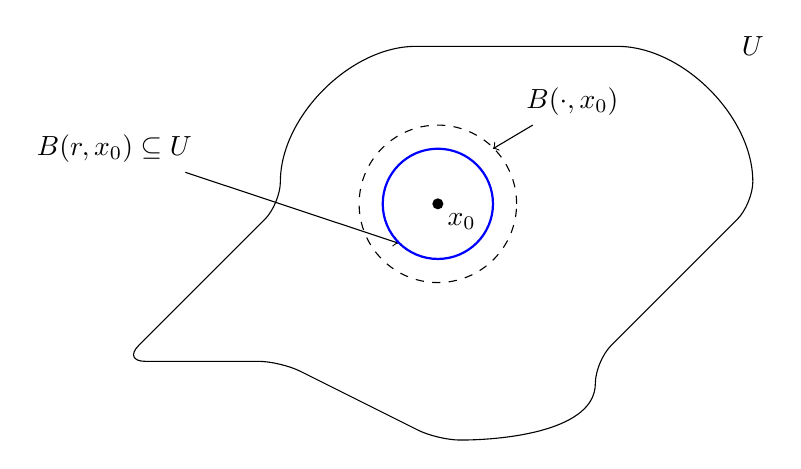
\begin{tikzpicture}
        % Draw the open set U
        \draw[rounded corners=8pt] (0,0) -- (2,2) to[out=90,in=180] (4,4) -- (6,4) to[out=0,in=90] (8,2) -- (6,0) to[out=-90,in=0] (4,-1) -- (2,0) -- cycle;

        % Label the set U
        \node at (8,4) {$U$};

        % Draw the point x
        \fill (4,2) circle (2pt);
        \node[below right] at (4,2) {$x_0$};

        % Label
        \node[above right] at (5,3) (ball) {$B(\cdot, x_0)$};
        \draw[->] (ball) -- (4.7,2.7);

        \node[below left] at (1,3) (ball) {$\cl{B(r, x_0)}\subseteq U$};
        \draw[->] (ball) -- (3.5 ,1.5);

        % Draw the open ball around x
        \draw[dashed] (4,2) circle (1);
        \draw[thick, blue] (4,2) circle (0.7);
        \end{tikzpicture}
        \caption{Every point $x_0$ in an open set $U$ admits an open ball that hides in $U$}
        \label{rudin-chp9-open set induces ball that hides inside}
    \end{figure}

    We claim the open ball $B(\lambda r, y_0)\subseteq V$. Indeed, suppose $y\in\realn$ with 
    \[
        d(y,y_0) < \lambda r
    \]
    If $\phi$ is the 'fixed-point detector' with respect to $y$ (the point we are trying to prove that is in $f(U)$), in fact: we will prove $y\in f(\cl{B(r,x_0)})\subseteq f(U)$.
    \[
        \underbracket{\phi(x_0) - x_0}_{\text{removing the offset from }\phi(x_0)} = A^{-1}(y - f(x_0)) = A^{-1}(y - y_0)
    \]
    using the operator norm on $A^{-1}(y-y_0)$ reads
    \[
        \norm{\phi(x_0) - x_0} = \norm{A^{-1}(y-y_0)}\leq \norm{A^{-1}}\norm{y-y_0}\leq \norm{A^{-1}}\lambda r = r2^{-1}
    \]
    We will drag $y$ into the image of the closed ball as follows: suppose $x$ is another point that lies in the closed ball, $\phi$ is contractive on $\cl{B}\subseteq U$ regardless of the point $y$ that induces $\phi$. But $\cl{B}$ is closed, hence it is complete. So the Cauchy sequence (from the contractive mapping theorem) produces exactly one point in $\cl{B}$. It remains to show that if we start our sequence at some point $x\in \cl{B}$, then $\phi(x)\in\cl{B}$ as well, and a simple induction will produce our contractive sequence.\\


    To this, fix $x\in \cl{B}$, and 
    \begin{align*}
        |\phi(x)-x_0|&\leq |\phi(x)-\phi(x_0)| + |\phi(x_0)-x_0|\\[1ex]
        &\leq \overbracket{2^{-1}|x-x_0|}^{\text{contraction on } \cl{B}\subseteq U} + \overbracket{r2^{-1}}^{\text{earlier}} \\[1ex]
        &= r
    \end{align*}
    therefore $\phi$ contracts to a fixed point $x^*\in \cl{B}$, and $f(x^*)=y$. So $y\in f(\cl{B})\subseteq f(U)$ as desired.
\end{proof}
\begin{proof}[Proof of Part B]
    The proof is quite long, and we will only focus on the important bits. Rudin uses the technique of approximating smooth functions using first-order terms. He writes
    \[
        \begin{cases}
            f(x) &= y \\
            f(x+h) &= y+k
        \end{cases}
        \implies k = f(x+h) - f(x)
    \]
    Furthermore, if $x\in U$, then the derivative $Df(x)$ is invertible, this is from Theorem 9.8, obtains an estimate on the open ball in $GL(n,\real)$. Roughly speaking, this open ball 'drags' other matrices into $GL(n,\real)$. If $A$ is invertible, and $B$ is a conformable matrix with $A$, then
    \[
    \underbracket{\norm{B-A}}_{\substack{\text{distance} \\ \text{between}\\ A, B}}\norm{A^{-1}}<1\implies B\in GL(n,\real)
    \]
    If $x\in B(\delta, a)$, then \Cref{rudin-chp9-24-derivative-bounded} reads 
    \[
        \norm{Df(x) - A}<\lambda\implies \norm{Df(x) - A}\norm{A^{-1}}<2^{-1}<1
    \]
    so $Df(x)$ is invertible with inverse $T$.\\

    And we estimate the deviation $|k|^{-1}\leq \lambda|h|^{-1}$ by using the contraction inequality with $y$ as the basepoint for $\phi$. Skipping a few lines ahead (to the confusing part), we see that
    \[
        |h|\leq |h-A^{-1}k| + |A^{-1}k|\leq 2^{-1}|h| + |A^{-1}k|
    \]
    subtracting over, and multiplying across gives a upper bound on $|k|^{-1}$
    \[
        2^{-1}|h|\leq |A^{-1}k|\implies 2^{-1}|h|\leq\norm{A^{-1}}|k|\implies |k|^{-1}\leq \underbracket{\dfrac{2}{\norm{A^{-1}}}}_{\lambda}|h|^{-1}
    \]
    Notice $2\lambda\norm{A^{-1}}=1$, so $2/\norm{A^{-1}}=\lambda$. Finally, we 'factor out' $-T$ on the line just before the difference quotient.
    \begin{align*}
        \overbracket{g(y+k)-g(y) - Tk}^{\substack{\text{numerator in }\\ \text{difference quotient}}} &= h - Tk \\[1ex]
        &= -T\biggl(\underbracket{f(x+h) - f(x)}_{=k} - \underbracket{Df(x)h}_{=T^{-1}h}\biggr)
    \end{align*}
    We see that $T = Dg(y)$, indeed:
    \begin{align*}
        \dfrac{|g(y+k)-g(y)- Tk|}{|k|}&\leq\dfrac{\norm{T}}{\lambda}\dfrac{|f(x+h)-f(x)-Df(x)h|}{|h|}\\
        &\Lsim \dfrac{|f(x+h)-f(x)-Df(x)h|}{|h|} \\
        = \underbracket{o(h) = o(k)}_{|h|\Lsim |k|}\to 0
\end{align*}

Finally, $Df|U: U\to GL(n,\real)$ is a continuous mapping. By Theorem 9.8, $(Df|U)^{-1}: U\to GL(n,\real)$ is continuous as well. Therefore $g\in C^1(U,U)$, and $f|U$ is a $C^1$-diffeomorphism.
\end{proof}
\begin{remark}
    The inverse function theorem is extremely powerful. If a $f$ is a $C^1$ map from and into $\realn$, and the total differential of $f$ is full rank (hence invertible, as it is square) at some point $a\in\realn$, the theorem states three things:
    \begin{itemize}
        \item For points $x$ within a small enough neighbourhood $a$, the total differential $Df(x)$ is invertible,
        \item On this same neighbourhood (denoted by $U$), $f(U)$ is a bijection,
        \item the inverse of $f$ is a $C^1$ map. This makes $f|U$ a $C^1$-diffeomorphism
    \end{itemize}
\end{remark}

\topheader{Inverse Function Theorem on Manifolds}
Let $F$ be a smooth map between two smooth manifolds $M$ and $N$, with dimensions $m$ and $n$ respectively.

% Rank, constant rank, smooth submersion,, smooth immersion

\begin{definition}[Rank of a map]
    The rank of $F$ at $p\in M$ is the rank of the linear map:
\[
    dF_p: T_pM\to T_{F(p)}N
\]\end{definition}

\begin{definition}[Constant rank maps]
A smooth map $F\in \cinf[M,N]$ has constant rank if its differential $dF_p: T_pM\to T_{F(p)}N$ has the same rank at every point $p\in M$.\end{definition}

There are three types of constant rank maps that are of interest. 
\begin{definition}[Smooth submersion]\label{lee-chp4:smooth-submersion-definition}
    $F$ is a smooth submersion if $dF_p$ is a surjection onto $T_{F(p)}N$ at $p$-everywhere. That is, $\rank dF_p = \dim T_{F(p)}N = \dim N$\end{definition}

\begin{definition}[Smooth immersion]\label{lee-chp4:smooth-immersion-definition}
    $F$ is a smooth immersion if $dF_p$ is an injection onto $T_{F(p)}N$ at $p$-everywhere. That is, $\rank dF_p = \dim T_{p}M = \dim M$\end{definition}


\begin{definition}[Smooth embedding]\label{lee-chp4:smooth-embedding-definition}
    $F$ is a smooth embedding if it is a smooth immersion, and it is a topological homeomorphism onto its range $F(M)\subseteq N$. 
\end{definition}

\begin{definition}[Topological embedding]\label{lee-chp4:topological-embedding}
    $F\in C(\xx,\yy)$, where $\xx$ and $\yy$ are topological spaces is a \emph{topological embedding} if $F$ is a homeomorphism onto its range.\\

    Inclusion maps are topological embeddings, as the restriction onto the range of the map is the identity.\\

    If $\xx$ is compact and $F$ is injective, then $F$ is a topological embedding. If $F$ is injective and an open map, then $F$ is a topological embedding as well.
\end{definition}

\begin{definition}[Topological submersion]\label{lee-chp4:topological-submersion}
    
\end{definition}

\begin{definition}[Local diffeomorphism]\label{lee-chp4:local-diffeomorphism-definition}
    $F$ is a local diffeomorphism if every $p\in M$ in its domain induces a neighbourhood $U\subseteq M$, $F(U)$ is open in $N$ with $F|U:U\to F(U)$ is a diffeomorphism (in the sense of two open sub-manifolds).
\end{definition}

\begin{wts}[Rank as an open condition]\label{lee-chp4:rank-open-condition-prop-4.1}
    Suppose $F: M\to N$ is a smooth map, and $p\in M$. If $dF_p$ is a surjection (resp. injection), pointwise at $p$, there exists a neighbourhood $U$ of $p$ where $F|U$ is a smooth submersion (resp. immersion)
\end{wts}
\begin{proof}
    Trivial. See \Cref{lee-chp4:example-1.28-matrices-of-full-rank}.
\end{proof}
Proposition 4.1 roughly states that, if the differential of $F$ at some point $p$ is injective or surjective, then there exists a neighbourhood $U$ about $p$ such that $dF|U(p)$ is an injection or surjection. The continuity of the map $dF|U(p) \mapsto \Delta_{m\times m}(dF|U(p))$, induces a neighbourhood in the vector space of matrices about the differential $dF|U(p)$. This vector space is endowed with any of the equivalent norms on $\mcal(m\times n,\real)$, which is equivalent to the entrywise $2$-norm. Since all partials of the form $\eval{\pdv{\hat{F}^{k}}{x^j}}_{\hat{p}}$ are continuous, we take the intersection over all $n\times m$ partials such that $dF|U(p)$ is an injection or surjection. Finally, send this neighbourhood about $\hat{p}$ through to $p$ by using the continuity of $\phi$.

\begin{wts}[Inverse Function Theorem on Manifolds]\label{lee-chp4:inverse-theorem-on-manifolds}
    Let $M$ and $N$ be smooth manifolds, and $F:M\to N$ be a smooth map. Suppose the differential of $F$ is invertible at some point $p\in M$, then there exists connected neighbourhoods $U_0$ of $p$, and $V_0$ of $F(p)$ such that $F|U_0:U_0\to V_0$ is a diffeomorphism.
\end{wts}
\begin{proof}
    Trivial. See the regular inverse function theorem \Cref{rudin-chp4-theorem-9.24} on Euclidean space, and pass the argument back to the manifolds using coordinate charts.
\end{proof}
\begin{wts}[Rank Theorem for Manifolds]\label{lee-chp4:rank-theorem-for-manifolds}
    Let $F:M\to N$ be a smooth map with constant rank $r$, then at every $p\in M$, there exists smooth charts $p\in (U,\phi)$ and $F(U)\subseteq(V,\psi)$, where the coordinate representation of $F$ takes the form
    \begin{align}\label{lee-chp4:rank-theorem-regular-case-coordinate-representation}
        \hat{F}(x) &= \begin{bmatrix}
            \id{r\times r} & 0_{r\times m-r}\\
            0_{n-r\times r} & 0_{n-r\times m-r}
        \end{bmatrix}x, && \qq{or equivalently}\\[2ex]
        \hat{F}(x^1,\ldots,x^r,x^{r+1},\ldots,x^m)&=(x^1,\ldots,x^r)
    \end{align}
\end{wts}
\begin{proof}
    Tedious. However, some techinques are worth remembering:
    \begin{itemize}
        \item Passing the argument to the Euclidean case as usual,
        \item We are free to shrink the sizes of open cubes and balls, and exploit local compactness,
        \item Suppose we are given a matrix of size $m\times n$, which has rank $r$, then we can attach a sub-matrix to make it square and invertible, then rehearse the usual arguments with the Inverse Function Theorems \Cref{rudin-chp4-theorem-9.24,lee-chp4:inverse-theorem-on-manifolds} to obtain a neighbourhood small enough that preserves the rank of the square matrix. Then pass the argument back to the smaller sub-matrix.
    \end{itemize}
    The last bullet point is worth elaborating, suppose we are given a rectangular matrix, where $A$ is square and invertible. Take $z = (x,y)^T$ with dimensions that make the formulas below make sense.
    \[
        Mz = \begin{bmatrix}
            A & B
        \end{bmatrix}\begin{bmatrix}
            x\\ y
        \end{bmatrix}\implies \begin{bmatrix}
            M\\ I
        \end{bmatrix}(z,y)^T = \begin{bmatrix}
            A & B\\ 0 & I
        \end{bmatrix}\begin{bmatrix}
            z\\ y
        \end{bmatrix}\qqtext{is square and invertible}
    \]
    by \Cref{lee-chp4:rank-open-condition-prop-4.1}, we see that there exists a neighbourhood about the square matrix $\begin{bmatrix} M\\ I\end{bmatrix}$ such that it remains invertible, hence a neighbourhood about $M$ that makes $A$ invertible (as a sub-matrix), so the rank of $M$ is preserved.
\end{proof}
\begin{corollary}[Rank Theorem for Manifolds - Special Cases]
    Let $F: M\to N$ be a smooth map with constant rank. If $F$ is a smooth immersion, then \Cref{lee-chp4:rank-theorem-regular-case-coordinate-representation} takes the form:
    \begin{align}\label{lee-chp4:rank-theorem-smooth-immersion-case-coordinate-representation}
        \hat{F}(x) &= \begin{bmatrix}
            \id{m\times m} \\
            0_{n-m\times m} 
        \end{bmatrix}x, && \qq{or equivalently}\\[2ex]
        \hat{F}(x^1,\ldots,x^m)&=(x^1,\ldots,x^m,0\ldots,0)
    \end{align}
    If $F$ is a smooth submersion,
    \begin{align}\label{lee-chp4:rank-theorem-smooth-submersion-case-coordinate-representation}
        \hat{F}(x) &= \begin{bmatrix}
            \id{n\times n} & 0_{n\times m-n}
        \end{bmatrix}x, && \qq{or equivalently}\\[2ex]
        \hat{F}(x^1,\ldots,x^n,x^{n+1},\ldots,x^m)&=(x^1,\ldots,x^n)
    \end{align}
    
\end{corollary}
\topheader{More on immersions and embeddings}
\begin{wts}[Characterization of smooth immersions]\label{lee-chp4:characterization-smooth-immersion}
    $F$ is a smooth immersion iff every point $p\in M$ has a neighbourhood $U\subseteq M$ where $F|U:U\to N$ is a smooth embedding.
\end{wts}
\begin{proof}
    We will prove it for when $M$ and $N$ are smooth manifolds, see Lee for the full proof with boundary. It involves extending the argument by composing $F$ with an inclusion map. From Lemma 3.11 (Lee), if $a\in \partial\halfn$, then the differential of the inclusion map $\iota:\halfn\to\realn$ is a linear isomorphism between tangent spaces.
    \[
        d\iota_a:T_a\halfn\to T_a\realn,\quad \underbracket{T_a\halfn\cong T_a\realn}_{\text{isomorphic}}
    \]
    If for every $p\in M$, there exists a neighbourhood $U$ of $p$ with $F|U: U\to N$ a smooth embedding, then $dF|U_p$ has rank $m$, so $dF_p$ has rank $m$, and the differential is injective pointwise everywhere. Conversely, if $dF_p$ is a smooth immersion, the Rank Theorem (\Cref{lee-chp4:rank-theorem-for-manifolds}) tells us there exists connected neighbourhoods of $p$ and $F(p)$, where $F$ has coordinate representation in \Cref{lee-chp4:rank-theorem-smooth-immersion-case-coordinate-representation} with respect to an appropriate choice of coordinate charts centered at $p$, so $\hat{F}(\hat{p})=0\in\realn$. Let $\hat{p}\in \hat{U}$ and $\hat{F}(\hat{p})\in \hat{V}$, the proof then devolves into a linear-map problem. $\hat{F}$ given by the expression in \Cref{lee-chp4:rank-theorem-smooth-immersion-case-coordinate-representation} is clearly injective. Therefore it is bijective onto its range, its inverse is nothing but the map that removes the extra zeroes at the end. Therefore $F|U$ is a smooth embedding.
\end{proof}
\begin{definition}[Section of $\pi: M\to N$]\label{lee-chp4:section-of-continuous-map}
   If $\pi: M\to N$ is a continuous map, a \emph{section of $\pi$} is a continuous right inverse for $\pi$, i.e $\sigma:N\to M$, $\sigma\in C(N,M)$, $\pi\circ\sigma=\id{N}$.\\

   A \emph{local section for $\pi$} is a continuous function $\sigma$ from an open set $U\subseteq V$ into $M$ with $\pi\circ\sigma=\id{U}$. 
\end{definition}

\begin{wts}[Characterization of smooth submersion]\label{lee-chp4:characterization-of-smooth-submersion}
    Let $\pi:M\to N$ be smooth, then $\pi$ is a smooth submersion iff every point of $M$ is in the image of a smooth local section of $\pi$.
\end{wts}
\begin{proof}
    Suppose $\pi$ is a smooth submersion, and fix $p\in M$, by the Rank Theorem \Cref{lee-chp4:rank-theorem-for-manifolds}, and \Cref{lee-chp4:rank-theorem-smooth-submersion-case-coordinate-representation}, $\pi$ has the coordinate representation
    \[
        \hat{\pi}(x^1,\ldots,x^n,x^{n+1},x^m)=(x^1,\ldots,x^n)
    \]
    between two open sets $U\subseteq M$ and $V\subseteq N$, (it really does not matter). Now, define
    \[
        \sigma: V\to M, (x^1,\ldots,x^n)\mapsto \underbracket{(x^1,\ldots,x^n,0,\ldots,0)}_{\realm}\in U
    \]
    the charts by assumption are centered, and $\pi\circ\sigma$ is clearly smooth (check coordinatewise), so $\sigma$ reaches $p$. Conversely, recall if the composition of maps $(g\circ f)$ is a surjection, then $g$ is a surjection. Now, fix $p\in M$, this induces an open set $V$ containing $\pi(p)$, and a smooth local section $\sigma_V: V\to M$. By \Cref{lee-chp3:properties-of-differential}, \emph{the differential of a composition is equal to the composition of the differentials}
    \[
        \id{T_{q}N}=d(\id{U})=d(\pi)_{\sigma(q)}\circ d(\sigma)_{q}
    \]
    so $d(\pi)_{\sigma{q}} = d(\pi)_{p}$ is a surjection and the proof is complete.
\end{proof}

\topheader{Regular values and level sets}
If $F:\xx\to\yy$, and $c\in \yy$, we call the $F^{-1}(\{y\})$ a \emph{level set at $c$}, and $c$ the \emph{level value}. We often write $F^{-1}(y)$ in place of $F^{-1}(\{y\})$. If $\yy=\realk$, then $F^{-1}(0)$ is the \emph{zero set of $F$}.

\begin{definition}[Critical point of {$F\in\cinf[N,M]$}]
    $p\in M$ is a \emph{critical point} of $F$ if the differential $dF_p:T_pN\to T_{F(p)}M$ fails to be surjective at $p$, otherwise $p$ is a \emph{regular point} of $F$.
\end{definition}
\begin{definition}[Critical value of {$f\in\cinf[N,\real]$}]
    Let $f$ be a test function on $N$, $c\in\real$ is a critical value if there exists a $p\in f^{-1}(c)$ where $df_p$ is not surjective.\\

    Otherwise $c$ is called a regular value. Caveat: if $c$ is not in the image of $f$, we call $c$ a regular value as well. It is clear $c$ is a regular value iff $c\notin f(M)$ or for every $p\in f^{-1}(c)$, $df_p$ is a surjection.\\

    Notice $df_p: T_pN\to T_{f(p)}\real$ is not surjective $\iff$ all partials of the coordinate representation of $f$ vanish. Since the matrix representation of $df_p$ has the form
    \[
        \mcal\{df_p\}=\mqty[\eval{\pdv{f}{x^1}}_{p} & \ldots & \eval{\pdv{f}{x^m}}_{p}]
    \]
    $\rank\mcal\{df_p\}\neq 1 \iff \eval{\pdv{f}{x^j}}_{p}=0$ for $1\leq j\leq m$.
\end{definition}
\begin{definition}[Regular level set of ${f\in\cinf[N,\real]}$]
    If $c$ is a regular value of $f$, then $f^{-1}(c)$ is called a regular level set.\\

    Define $g = f-c$, the partials at $p\in N$ for both $f$ and $g$ agree, so the matrix representations of $df_p$ and $dg_p$ are identical (whereas their ranges might not be),
    \begin{align*}
        \mcal\{dg_p\}&=\mqty[\eval{\pdv{g}{x^1}}_{p} & \ldots & \eval{\pdv{g}{x^m}}_{p}]\\[2ex]
        &=\mqty[\eval{\pdv{f-c}{x^1}}_{p} & \ldots & \eval{\pdv{f-c}{x^m}}_{p}]\\[2ex]
        &=\mqty[\eval{\pdv{f}{x^1}}_{p} & \ldots & \eval{\pdv{f}{x^m}}_{p}]\\[2ex]
        &= \mcal\{df_p\}
    \end{align*}
\end{definition}

\topheader{Submanifolds}
\begin{definition}[Embedded submanifold of $M$]\label{lee-chp5:embedded-submanifold}
    A subset $S$ of $M$ is called an \emph{embedded submanifold of $M$}, when:
    \begin{itemize}
        \item equipped with the subspace topology from $M$,
        \item it has a smooth structure that makes it a smooth manifold, and
        \item the inclusion map $\iota: S\hookrightarrow M$ is a smooth embedding.
    \end{itemize}
\end{definition}


\begin{definition}[Immersed submanifold of $M$]\label{lee-chp5:immersed-submanifold}
    A subset $S$ of $M$ is called an \emph{immersed submanifold of $M$}, when:
    \begin{itemize}
        \item equipped with an \emph{arbitrary topology},
        \item it has a smooth structure that makes it a smooth manifold (with or without boundary), and
        \item the inclusion map $\iota: S\hookrightarrow M$ is a smooth immersion.
    \end{itemize}
\end{definition}


\begin{definition}[Properly embedded submanifold]\label{lee-chp5:properly-embedded-submanifold}
    is an embedded submanifold, and the inclusion map $\iota:S \to M$ is a \emph{proper} map. 
\end{definition}

\begin{definition}[Weakly embedded submanifold]\label{lee-chp5:weakly-embedded-submanifold}
    is an immersed submanifold of $M$, whenever $F:N\to M$ is a smooth map and the range of $F$ lies in $S$, then $F:N\to S$ as a map between two manifolds.
\end{definition}


\topheader{Measure zero}
\begin{definition}[Measure zero]\label{lee-measure-zero}
    A subset $E\subseteq\realn$ has \emph{measure zero} if $\mu(E)=0$
    \[
        \mu(E) = \inf\bigset{\sum_{j\geq 1} m(U_j),\: E\subseteq \bigcup U_j,\: U_j\in\mcal}
    \]
    where $\mcal$ denotes the Borel $\sigma$-algebra on $\realn$. Each $U_j$ can be taken to be open/closed balls or cubes, as they are measurable.\\

    We sometimes refer to a measure zero set as \emph{null}. If $M$ is a smooth manifold of dimension $m$, then $E\subseteq M$ has \emph{measure zero} if for every chart $(U,\varphi)\in\mathcal{A}_M$, 
    \[
        \varphi(U\cap E)\subseteq\realm\quad\text{has measure zero in }\realm
    \]
\end{definition}
\begin{wts}[Subadditivity and Monotonicity of null sets]\label{lee-sards-subadditivity}
    The countable union of null sets is again null. Any measurable subset of a null set is again null. This holds for $\realn$ and the smooth manifold case.
\end{wts}
\begin{proof}
    See any textbook on the theory of integration.
\end{proof}
\begin{wts}[Slice criterion for measure zero]\label{lee-theorem6.2}
    Suppose $A\subseteq\realn$ is compact (not necessary), and for every $c\in \real$, define the $c$-section of $A$
    \[
        A_c = \bigset{x\in\real^{n-1},\: (c,x)\in A}
    \]
    If $A_c$ has measure zero in $\real^{n-1}$ for every $c\in\real$, then $A$ has measure zero
\end{wts}
\begin{proof}
    By Tonelli's Theorem, since the Lebesgue measure on $\borel_\realn$ is a Radon measure, it is finite on compact sets. Hence
    \[
        \mu(A)=\int fd\mu_n = \int \chi_{A}d\mu_1\times\cdots\times\mu_n
    \]
    where $f(c) = \int \chi_{A_c}d\mu_1\times\cdots\times\mu_{n-1}$ is $0$ for all $c$, hence $\int fd\mu_n$ integrates to zero.
\end{proof}
\begin{wts}[Equivalent condition for manifold measure zero]\label{lee-theorem6.6}
    Let $E\subseteq M$, if $\{(U_\alpha,\: \varphi_\alpha)\}$ is a collection of charts that cover $A$, and $\varphi_\alpha(E\cap U_\alpha)$ has measure zero for every $\alpha$, then $E$ has measure zero.
\end{wts}

\begin{wts}[Smooth maps send null sets to null sets]\label{lee-theorem6.9}
    If $F\in\cinf[M,N]$, and $A\subseteq M$ has measure zero, so does $F(A)$. In particular, this holds for $F\in\cinf[\realm,\realn]$ with the standard smooth structures.
\end{wts}

\topheader{Lemmas for Sard's Theorem}

\begin{lemma}[Lemmas on regular/critical points]\label{lee-regular-critical-points}
    Let $M$ and $N$ be smooth manifolds, and $F\in\cinf[M,N]$. Then,
    \begin{enumerate}
        \item The set of regular points of $F$ are open in $M$.
        \item The set of critical points of $F$ are closed in $M$.
        \item The set of critical values of $F$ are precisely the direct image of its critical points. In symbols:
        \begin{equation}\label{lee-critical-values-image-of-critia-points}
            \text{Critical Values} = F(\text{critical points})
        \end{equation}
    \end{enumerate}
\end{lemma}
\begin{lemma}[Local characterization of critical points]\label{lee-critical-points-local}
    Let $p\in M$, and if $p\in (U,\varphi)$, $F(U)\subseteq(V,\psi)$. Then the rank of $dF_p$ is independent of the choice of coordinate charts used, and it is equal to the rank of $d\hat{F}_{\hat{p}}$. Where $\hat{F}$ is the coordinate representation of $F$ with respect to the charts $(U,\: \varphi)$ and $(V,\psi)$.
        \[
            \hat{F}:\varphi(U)\to\psi(V)\quad \hat{F}\defined \psi\circ F\circ \varphi^{-1}
        \]
    Moreover, if $p$ a critical point of $F$, it is also a critical point of $F|_{U'}:U'\to V'$. Where $U'$ is an open subset of $U$, and $V'$ is an open subset of $V$ that contains $F(U')$ entirely.
\end{lemma}
\begin{lemma}[LCH Lemma for Sard's Theorem]\label{lee-sards-LCH}
    Let $\xx$ be a LCH space. Suppose $x\in \xx$, and $U$ is an open set containing $x$. There exists an open precompact neighbourhood about $x$ that \emph{hides in $U$}. If $V$ denotes this neighbourhood, then
    \[
        x\in V\subseteq\cl{V}\subseteq U
    \]
\end{lemma}

\begin{lemma}[Covering Lemmas for Sard's Theorem]\label{lee-covering-lemmas}
    The following holds for an arbitrary $m$.
    \begin{enumerate}
        \item If $U\subseteq\realm$ is an open set, it can be covered by
        \begin{itemize}
            \item countably many open balls, 
            \item countably many open cubes,
            \item countably many closed balls,
            \item countably many closed cubes,
        \end{itemize}
        all of the above are subsets of $U$.
        \item If $E\subseteq\realm$ is a closed cube with side length $R$, then it can be covered by $K^m$ many closed cubes with equal side lengths $R'=RK^{-1}$.
    \end{enumerate}
\end{lemma}

\begin{lemma}[Diffeomorphism invariances for Sard's Theorem]\label{lee-diffeomorphisms-invariance}
    Let $M$, $N$, $P$, $Q$ be smooth manifolds. Let $F\in\cinf[M,N]$, and $G\in\diffeo[M,M]$,
    \begin{enumerate}
        \item If $p\in M$, define $H = F\circ G$, then
        \begin{itemize}
            \item $\rank dF_p = \rank dH_p$,
            \item $p$ is a critical point of $F$ iff it is a critical point of $H$,
            \item $E\subseteq M$ has measure zero iff $G(E)$ has measure zero,
            \item topological properties are preserved (applies for homeomorphisms $G$). $E$ is compact, open, closed, connected or path-connected iff $G(E)$ is.
        \end{itemize}
        \item Let $H\in\diffeo[Q,M]$, if $U$ is an open subset of $Q$, then $H|_{U}:U\to H(U)$ is again a diffeomorphism, where $U$ and $H(U)$ are interpreted as open-submanifolds of $Q$ and $M$.
    \end{enumerate}
\end{lemma}

\topheader{Sard's Theorem}

\begin{wts}[Sard's Theorem]
    Let $M$ and $N$ be smooth manifolds with dimensions $m$ and $n$, then the set of critical values of $F$ has measure-zero in $N$.
\end{wts}
The proof for Sard's Theorem is extremely long. We will use induction on the dimension of $M$. The base case will be divided into two sub-cases, one where $n=0$ and $n\geq 1$.\\


\begin{step}[Base case: $m = 0$]
    Let $G\in\cinf[P,N]$ where $P$ and $N$ are smooth manifolds with dimensions $p = 0$ and $n\geq 1$. The set of critical values of $G$ have measure zero in $N$.
\end{step}


As we will soon see, the induction hypothesis allows  us to use several dimension reduction techniques to prove the induction step. These techniques will depend on the rank theorem.
\begin{step}[Induction hypothesis]
    Let $G\in\cinf[P,N]$ where $P$ and $N$ are smooth manifolds with dimensions $0\leq p\leq m-1$ and $n\geq 1$. The set of critical values of $G$ have measure zero in $N$.
\end{step}

The induction step is extremely fussy. First, we dissect the domain and range of $M$ and $N$ into countably many charts $\{((U_{jk}, \varphi_{jk}),(V_{jk},\psi_{jk})\}_{j,k\geq 1}$ where

\begin{equation}\label{lee-sards-Ujk-Vjk-spec}
    F(U_{jk})\subseteq V_{jk}    
\end{equation}
that also cover $M$ and $N$. \\

By \Cref{lee-critical-points-local}, if $p$ is a critical point of $F$ and $p\in U_{jk}$, then $p$ is a critical point of 
\begin{equation}\label{lee-sards-Fjk-spec}
    F_{jk}: U_{jk}\to V_{jk}
\end{equation}

\begin{step}[Construction of charts]\label{lee-sards-construction-charts}
    We construct a countable sequence of $\{((U_{jk}, \varphi_{jk}),(V_{jk},\psi_{jk})\}_{j,k\geq 1}$ charts that satisfy \Cref{lee-sards-Ujk-Vjk-spec,lee-sards-Fjk-spec}.
\end{step}
\begin{proof}
    Let $\{(U_\alpha, \varphi_\alpha)\}$ be the maximal smooth atlas on $M$. Each $U_\alpha$ is open in $M$, and $M$ is second-countable. It follows that there exists a countable open cover (indexed by $j\geq 1$) that covers $M$, and a countable smooth atlas $\{(U_j, \varphi_j)\}$. Similarly for $\{(V_k,\psi_k)\}$.\\

    Let us write $U_{jk}\defined U_j\cap F^{-1}(V_k)$. Note $U_{jk}$ is open, since smoothness implies continuity (Proposition 2.4). And
    \[
        (V_{jk}, \psi_{jk})\defined (V_k, \psi_k)\quad F_{jk}=F|_{U_{jk}}
    \]
    so $F_{jk}(U_{jk})\subseteq V_{jk}$. Finally, define $\varphi_{jk}=\varphi_j|_{U_{jk}}$.
\end{proof}

Using \Cref{lee-theorem6.9}, smooth maps preserve measure-zero sets. If the critical values of some $F_{jk}$ have measure zero in $N_{jk}$, then so does $\iota(\text{critical points of } F_{jk})$, where is the smooth $\iota: N_{jk}\hookrightarrow N$ is the inclusion map (which is a smooth embedding by \Cref{lee-chp5:embedded-submanifold}). Thus,

\begin{step}[Pass the measure-zero condition to each chart]
    Prove the following
    \begin{align*}
    &F(\text{critical points of } F)\: \text{has measure zero}
    \\ &\iff
    \text{For } j,k\geq 1,\quad F_{jk}(\text{critical points of }F_{jk})\:\text{ null in } V_{jk}\subseteq N
    \\&\iff 
    \text{For } j,k\geq 1,\quad \hat{F}_{jk}(\text{critical points of }\hat{F}_{jk})\:\text{ null in } \psi_{jk}(V_{jk})\subseteq \realn
\end{align*}

where $\hat{F}_{jk}$ denotes the coordinate representation of $F$ with respect to the charts $(U_{jk}, \varphi_{jk})$ and $(V_{jk},\psi_{jk})$.
\begin{equation}
    F_{jk}:\varphi_{jk}(U_{jk})\to \psi_{jk}(V_{jk}),\quad \hat{F}_{jk}\defined \psi_{jk}\circ F_{jk}\circ \varphi_{jk}
\end{equation}
\end{step}
\begin{proof}
    The first equivalence follows from \Cref{lee-critical-points-local}, and the observation that the image of $F$ commutes with unions. The second follows from \Cref{lee-theorem6.9,lee-diffeomorphisms-invariance}.
\end{proof}


To simplify the problem even further, we assume $U_{jk}$ and $V_{jk}$ are open subsets of $\realm$ and $\realn$, as the core of the 'measure-zero' argument is invariant under diffeomorphisms of the coordinate charts (see \Cref{lee-diffeomorphisms-invariance}). Let $j,k$ be fixed, and relabel
\[
    ((U_{jk},\varphi_{jk}),\: (V_{jk},\psi_{jk}))\mapsto ((U,\varphi),\: (V,\psi))\qqtext{and} F_{jk}\mapsto F
\]
similarly for $\hat{F}_{jk}\mapsto \hat{F}$.

\begin{step}[Pass measure-zero condition to {$\realm$} and {$\realn$}]
    Let $U$ and $V$ be open sub-manifolds of $M$ and $N$, and $\varphi$ and $\psi$ be global (smooth) charts.
    \[
        F(\text{critical points of } F) = (\psi^{-1}\circ \hat{F}\circ \varphi)(\text{critical points of }F)
    \]
    and
    \[
        \text{critical points of }F = \varphi^{-1}(\text{critical points of } \hat{F})
    \]
\end{step}
\begin{proof}
    The first equation follows from the definition of $\hat{F}$, after unboxing the domains and ranges.
\end{proof}
We again relabel:
\[
    U\mapsto \varphi(U),\quad V\mapsto \psi(V),\quad F\mapsto \hat{F}
\]

and $M\mapsto \realm$, $N\mapsto \realn$, and critical points of $F$. Now $F: U\to V$ is a smooth map between open subsets of $\realm$ and $\realn$. Let us state the goal of the induction.
\begin{step}[Simplified induction goal]\label{lee-sards-simplified-induction-hypothesis}
    Let $U\subseteq\realm$ and $V\subseteq\realn$ be open subsets. $F\in\cinf[U,\realn]$ is a smooth map. Where $\realm$ and $\realn$ are considered to be smooth manifolds with the standard smooth structure. Prove that the set of critical values of $F$ have measure zero.
\end{step}

We define some standard notation for partials.
\begin{itemize}
    \item $\nat_0\defined\{0,1,\ldots\}$,
    \item $\alpha$ is a \emph{$m$-multi-index} or a \emph{multi-index of order $m$} if $\alpha = (\alpha_1,\ldots,\alpha_m)$ is a $m$-tuple with entries in $\nat_0$. The set of $m$-multi-indices are denoted by $\nat_0^m$.
    \item The order of a multi-index $\alpha$, denoted by $|\alpha|$ is its $l^1$ norm. In symbols:
    \[
        |\alpha|=\sum |\alpha_j|
    \]
    \item If $g\in\cinf[\realm,\real]$, and $\alpha\in\nat_0^m$, we define 
    \[
        \partial^\alpha g\defined \qty(\pdv{x^1})^{\alpha_1}\cdot\:\cdots\:\cdot\qty(\pdv{x^m})^{\alpha_m}
    \]
    so that $\partial^\alpha \defined \prod_{1}^m\qty(\pdv{x^j})^{\alpha_j} = \prod_{j=1}^m\partial_j^{\alpha_j}$.
\end{itemize}

Let $C\subseteq U$ denote the set of critical points of $F$, we decompose $F(C)$ into the following
\begin{equation}\label{lee-sards-decompose-C}
    F(C) = F(C\setminus C_1) + \bigcup_{j=1}^{k-1} F(C_j\setminus C_{j+1}) + F(C_k)
\end{equation}
    
and show each of the three sets in the union have measure zero. (the direct image commutes with unions). Where
\[
    C_k \defined\bigset{x\in C,\: \forall i\leq n,\:\alpha\in\nat_0^m,\:|\alpha|\leq k,\: \partial^\alpha F^i(x)=0}
\]
and $F^i$ are the \emph{component functions} of $F$, or $F(x) = (F^{1}(x),\ldots,\: F^{n}(x))$.


\begin{step}[Properties of $C$, $C_k$]
    $C$, $C_k$ is closed for every $k\geq 1$, and 
    $
    U\supseteq C\supseteq C_1\supseteq C_2\supseteq \cdots
    $.
\end{step}
\begin{proof}
    $C$ is closed by \Cref{lee-regular-critical-points}. The function 
    \[
        h(x)\defined \sum_{{\substack{\alpha\in\nat_0^m\\ |\alpha|\leq k\\ i=1,\ldots,n}}}|\partial^\alpha F^i(x)|
    \]
    is a continuous map from $U\to\real$. and $h^{-1}(0)\cap C$ is closed by continuity. $C\supseteq C_1$ follows by definition of $C_1$, and $C_k\supseteq C_{k+1}$ follows from comparing $h$ for the two values of $k$.
\end{proof}

\begin{step}[Case I: {$C\setminus C_1$} has measure zero.]\label{lee-sards-case1}
    
\end{step}
Let $a\in C\setminus C_1$, noting that $U\setminus C_1$ is an open set containing $a$. Since $a\notin C_1$, there exists a first order non-vanishing partial for a component function of $F$. Suppose 
\[
    \pdv{x^j}F^{i}(a)\neq 0\qqtext{with respect to the standard charts}
\]
We wish to swap the columns and rows of the coordinate charts so that $\pdv{x^1}F^{-1}(a)\neq 0$. More concretely, the transposition of the $i$th and the $1$st row is a permutation; so is the transposition of the $j$th and the $1$st column. By invariance, we are free to relabel
\[
    F\mapsto P_{i,1}\circ F\circ P_{j,1}
\]
Next, we use a convenient change of coordinates, to arrive at the form described below.
\begin{step}[Change of Coordinates]
    Perform a change of coordinates, such that if $(u,v^2,\ldots,v^m) = (u,v)$, where $v\in\real^{n-1}$, then
    \begin{equation}\label{lee-sards-eq-6.2a}
        F(u,v) = (u,F^2(u,v), \ldots, F^n(u,v))
    \end{equation}
    and the differential is given by
    \begin{equation}\label{lee-sards-eq-6.2b}
        dF_{(u,v)} = \begin{bmatrix}
            1&0\\ \eval{\pdv{F^i}{u}}_{(u,v)} & \eval{\pdv{F^i}{v^j}}_{(u,v)}
        \end{bmatrix}\quad \substack{i=2,\ldots,n\\ j=2,\ldots,m}
    \end{equation}
    where $dF_{(u,v)}$ is not surjective for each $(u,v)\in C\setminus C_1\subseteq C$. This change of coordinates is valid on some open, precompact set containing $a$, denoted by $V_a$. More precisely
    \begin{equation}\label{lee-sards-precompact}
    a\in V_a\subseteq\cl{V}_a\subseteq B\subseteq U\setminus C_1
    \end{equation}
\end{step}
\begin{proof}
If $(x^1,\ldots,x^m)$ are the standard coordinates of $\realm$, the map 
    \[
        T: (x^1,\ldots,x^m)\mapsto (F^1(a),x^2,\ldots,x^m)\quad\text{is a diffeomorphism}
    \]
    on some open, precompact neighbourhood $V_a$ of $a$.
    \[
        a\in V_a\subseteq \cl{V_a}\subseteq U
    \]
    
    The Jacobian of $T$ is given by
    \[
        \operatorname{Jacobian}(T)(x)=\begin{bmatrix}
            \pdv{F^1}{x^1}(x) & \cdots \\ * & Id_{m-1}
        \end{bmatrix}
    \]
    and it is invertible at $a$. The continuity of $\pdv{F^1}{x^1}$ at $a$ gives us an open ball $B\subseteq U\setminus C_1$ containing $a$, on which $\pdv{F^1}{x^1}\neq 0$. Let $V_a\subseteq\cl{V}_a\subseteq B$ be an open, precompact neighbourhood that hides in this ball as in \Cref{lee-sards-LCH}. \\

    Next, we absorb the change of coordinates into $F$, so
    \[
        F\mapsto (F\circ T^{-1})|_{B}
    \]
    Verification of the \Cref{lee-sards-eq-6.2a} is straightforward, as
    \[
    T^{-1}(u,v) = ((F^1)^{-1}(u,v), v^2,\ldots,v^m)
    \]
    \begin{align*}
        (F\circ T^{-1})(u,v) 
        &= \biggl(F^1[(F^1)^{-1}(u,v))], \ldots,\ldots\biggr)\\
        &= (u, F^2(u,v),\ldots, F^n(u,v))
    \end{align*}
    Computing the Jacobian matrix gives \Cref{lee-sards-eq-6.2b}, and $V_a$ clearly satisfies \Cref{lee-sards-precompact}.
\end{proof}

Let $a$ range through all points in $C\setminus C_1$, then $\{C\setminus C_1\cap V_a\}_{a\in C\setminus C_1}$ is an open cover Rel $C\setminus C_1$, so there exists a countable subcover. We will prove something slightly stronger, we prove that $F(C\setminus C_1\cap \cl{V_a})$ has measure zero for each $a$ in this countable collection. \Cref{lee-sards-subadditivity} will then prove $F(C\setminus C_1)$ is null.\\

Notice $C\setminus C_1\cap \cl{V_a}$ is a closed subset of $\cl{V_a}$, hence compact. Continuous functions send compact sets to compact sets, so $F(C\setminus C_1\cap \cl{V_a})$ is compact in $\realn$. We wish to use the induction hypothesis and 'lower the dimension' of $F$, or at the very least — pass the argument to a lower dimension.


\begin{step}[{$F(C\setminus C_1\cap \cl{V_a})$} has measure zero.]\label{lee-sards-case1-neighbourhoods}
    In this step, we show every point in $C\setminus C_1$, admits a neighbourhood which is null. So
    \[
        F(C\setminus C_1 \cap V_a)\subseteq F(C\setminus C_1\cap \cl{V}_a)
    \]
    $V_a$ is open Rel $C\setminus C_1$, and $a$ ranges through all the points in $C\setminus C_1$. $C\setminus C_1$ is second countable in the subspace topology, so $\{V_a\}$ admits a countable subcover, and we can apply subadditivity.
\end{step}
\begin{proof}
    Let $a$ an element in the countable subcollection described above. Let $c\in\real^{1}$ be arbitrary, if
    \[
        \{c\}\times\real^{n-1}\cap F(C\setminus C_1\cap \cl{V}_a)=\varnothing
    \]
    then the $c$-section $E_c$ of $F(C\setminus C_1\cap \cl{V}_a)$, 
    
    \[
    E_c \defined \{q\in \real^{n-1},\: (c,q)\in F(C\setminus C_1\cap \cl{V}_a)\}
    \]
    is empty, so $E_c$ is null. Next, if $E_c$ is not empty, we will pass the argument to some $F_c: \underbracket{B_c}_{\subseteq \real^{m-1}}\to \real^{n-1}$ and show $E_c$ is \emph{exactly} (double inclusion) the set of critical points of $F_c$. Indeed, define
    \[
        B_c = \bigset{v,\: (c,v)\in\cl{V}_a}\qqtext{and}F(c,v)=(c,F_c(v))
    \]
    so $F_c(v) = (F^2(c,v),\ldots,F^{n}(c,v))$ for $v\in B_c$. The Jacobian (differential) of $F_c$ resembles that of $F$. With $c$ fixed,
    \[
        (dF_c)_v = \begin{bmatrix}
            {v^j}_{(u,v)}
        \end{bmatrix}\quad \substack{i=2,\ldots,n\\ j=2,\ldots,m}
    \]
    Compare the previous equation with \Cref{lee-sards-eq-6.2b}, what we have done essentially is \emph{removing the first column and row} of $dF_{(c,v)}$. By elementary linear algebraic arguments about canonical forms, $\rank dF_{(c,v)}\neq n\iff \rank (dF_c)_v\neq n-1$. So $(c,v)\in C\setminus C_1\cap \cl{V}_a$ if and only if $v$ is a critical point of $F_c$.  If $(c,x)$ is a critical value in $C\cap \cl{V_a}$, then $DF$ cannot have full rank so 
    \[
        \qty[\pdv{F^i}{v^j}](x)\:\text{ as a function of }x\in\real^{n-1}\text{ cannot have full rank.}
    \]
    Now we wish to use the $c$-section Lemma in \Cref{lee-theorem6.2} in conjunction with our induction hypothesis. $C\setminus C_1\cap \cl{V}_a$ is a closed subset of compact $\cl{V}_a$, hence $F(C\setminus C_1\cap \cl{V}_a)$ is again compact. The $c$-section
    \[
        \qty[F(C\cap \cl{V}_a]_c = \bigset{x\in\real^{n-1},\: (c,x)\in F(C\cap\cl{V}_a)}
    \]
    so $(c,x)$ is a critical value of $F|_{\cl{V}_a}$. Another key idea is the following:
    \begin{itemize}
        \item Define $F_c(v) = (F^2(c,v),\ldots, F^n(c,v))$, 
        \item so $\eval{(DF_c)}_{v} = \qty[\pdv{F^i}{v^j}]$ from slicing the bottom right corner of the matrix in \Cref{lee-sards-eq-6.2b}.
        \item $\qty[F(C\cap \cl{V}_a)]_c = \bigset{x\in\real^{n-1},\: (c,x)\in F(C\cap \cl{V}_a)}$ 
    \end{itemize}
    
\end{proof}
This completes Case I. 

% Complete Case II and Case II for the proof of Sard's Theorem Later.

\topheader{Whitney Embedding Theorem}


\topheader{Whitney Approximation Theorems}

\topheader{Tubular Neighbourhood Theorem}

\topheader{Transversality}





\end{document}